\documentclass[10pt,twocolumn,a4paper]{article}
\usepackage[margin=1.8cm,columnsep=0.6cm]{geometry}
\usepackage[T1]{fontenc}
\usepackage{mathptmx}
\usepackage{amsmath,amssymb}
\usepackage{graphicx}
\usepackage{booktabs}
\usepackage{xcolor}
\usepackage[hidelinks]{hyperref}
\usepackage{caption}
\captionsetup{font=small,labelfont=bf}
\setlength{\parskip}{2pt}
\graphicspath{{../../results/}}
\newcommand{\overshoottext}{PID: 12.0\,\%, LQR: 2.7\,\%, MPC: 2.7\,\%, RL: 7.8\,\%}


\title{\vspace{-1.2cm}\textbf{Energy-Efficient Control of an Inverted Pendulum:\\
PID vs.\ LQR vs.\ MPC vs.\ Reinforcement Learning}}
\author{Amirreza Mohamadi and Reza Ghorbani\\
\small Technical report, team portfolio project, October 2026}
\date{}

\begin{document}
\maketitle

\begin{abstract}
We compare four controllers for balancing an inverted pendulum on a cart with
as little control energy as possible: a cascaded PID, a discrete LQR, a linear
MPC solved with CasADi/qpOASES, and a Soft Actor-Critic (SAC) policy. All four
run on the same validated nonlinear simulator with the same force limit,
control rate and initial conditions, and all are tuned for the same cost
$J = J_\mathrm{track} + \rho E_u$, sweeping the energy weight $\rho$ to trace
energy--accuracy Pareto fronts.
All controllers balanced the pendulum in every one of the $4\times20$ test
runs. LQR forms the Pareto front in all four scenarios; the linear MPC
reproduces LQR exactly whenever its constraints are inactive and only helps
near the track limits; the grid-searched PID comes close to the front; the
SAC policy needs 2--10$\times$ the tracking cost of LQR at equal energy in
nominal regulation, but beats the LQR front under a push disturbance it was
trained on.
\end{abstract}

\section{Introduction}
Every newton of actuator force drains the battery of a mobile robot, so a
controller that reaches the same accuracy with less effort directly extends
operating time. The inverted pendulum on a cart is the standard benchmark for
comparing control approaches: it is unstable, nonlinear and underactuated, yet
small enough to model by hand. We ask which of four controller families keeps
the pendulum upright with the least control energy \emph{at comparable
accuracy}. Because a controller can always save energy by being less accurate,
we report energy--accuracy Pareto fronts rather than a single ranking.

\section{System Model}
\textbf{Equations of motion.} With generalized coordinates $q=[x,\theta]^\top$
(cart position, pendulum angle, $\theta=0$ upright, positive towards $+x$), a
point-mass pendulum (mass $m$ at distance $l$ from the pivot) and no friction,
the Lagrange method gives
\begin{align}
\ddot x &= \frac{u + ml\dot\theta^2\sin\theta - mg\sin\theta\cos\theta}{M+m\sin^2\theta},\label{eq:xdd}\\
\ddot\theta &= \frac{(M+m)g\sin\theta - u\cos\theta - ml\dot\theta^2\sin\theta\cos\theta}{l\,(M+m\sin^2\theta)}.\label{eq:thdd}
\end{align}
The derivation was checked symbolically with SymPy. Parameters: $M=1$\,kg,
$m=0.1$\,kg, $l=0.5$\,m, $g=9.81$\,m/s$^2$, $|u|\le 10$\,N, $|x|\le 2.4$\,m,
$\Delta t=0.02$\,s. Note that Gymnasium's \texttt{CartPole-v1} uses the same
numbers but a uniform rod; our RL environment therefore wraps our own model.

\textbf{Linearization.} Around the upright equilibrium, with
$s=[x,\dot x,\theta,\dot\theta]^\top$,
\begin{equation}
A=\begin{bmatrix}0&1&0&0\\0&0&-\frac{mg}{M}&0\\0&0&0&1\\0&0&\frac{(M+m)g}{Ml}&0\end{bmatrix},\;
B=\begin{bmatrix}0\\\frac1M\\0\\-\frac{1}{Ml}\end{bmatrix},
\end{equation}
i.e.\ $A_{24}=-0.981$, $A_{43}=21.58$, $B=[0,1,0,-2]^\top$, with an unstable
pole at $+4.65$\,rad/s (the angle error doubles every 0.15\,s). Zero-order-hold
discretization at 50\,Hz gives $(A_d,B_d)$.

\textbf{Simulator and validation.} The force is held constant over each
20\,ms period and the nonlinear model is integrated with 10 classical RK4
substeps. The simulator, not the controller, clips $u$ to $\pm10$\,N.
Validation: (i)~with $u=0$ a pendulum tilted by $5^\circ$ falls past
$90^\circ$ after 0.80\,s; (ii)~total energy drifts by only
$1.4\cdot10^{-10}$\,J over 10\,s and horizontal momentum stays zero;
(iii)~the RK4 error shrinks by more than $16\times$ per halving of the step;
(iv)~$A,B$ equal the numerical Jacobian of \eqref{eq:xdd}--\eqref{eq:thdd};
(v)~linear and nonlinear responses differ by $0.02^\circ$ at $\theta=10^\circ$.

\begin{figure*}[t]
\centering
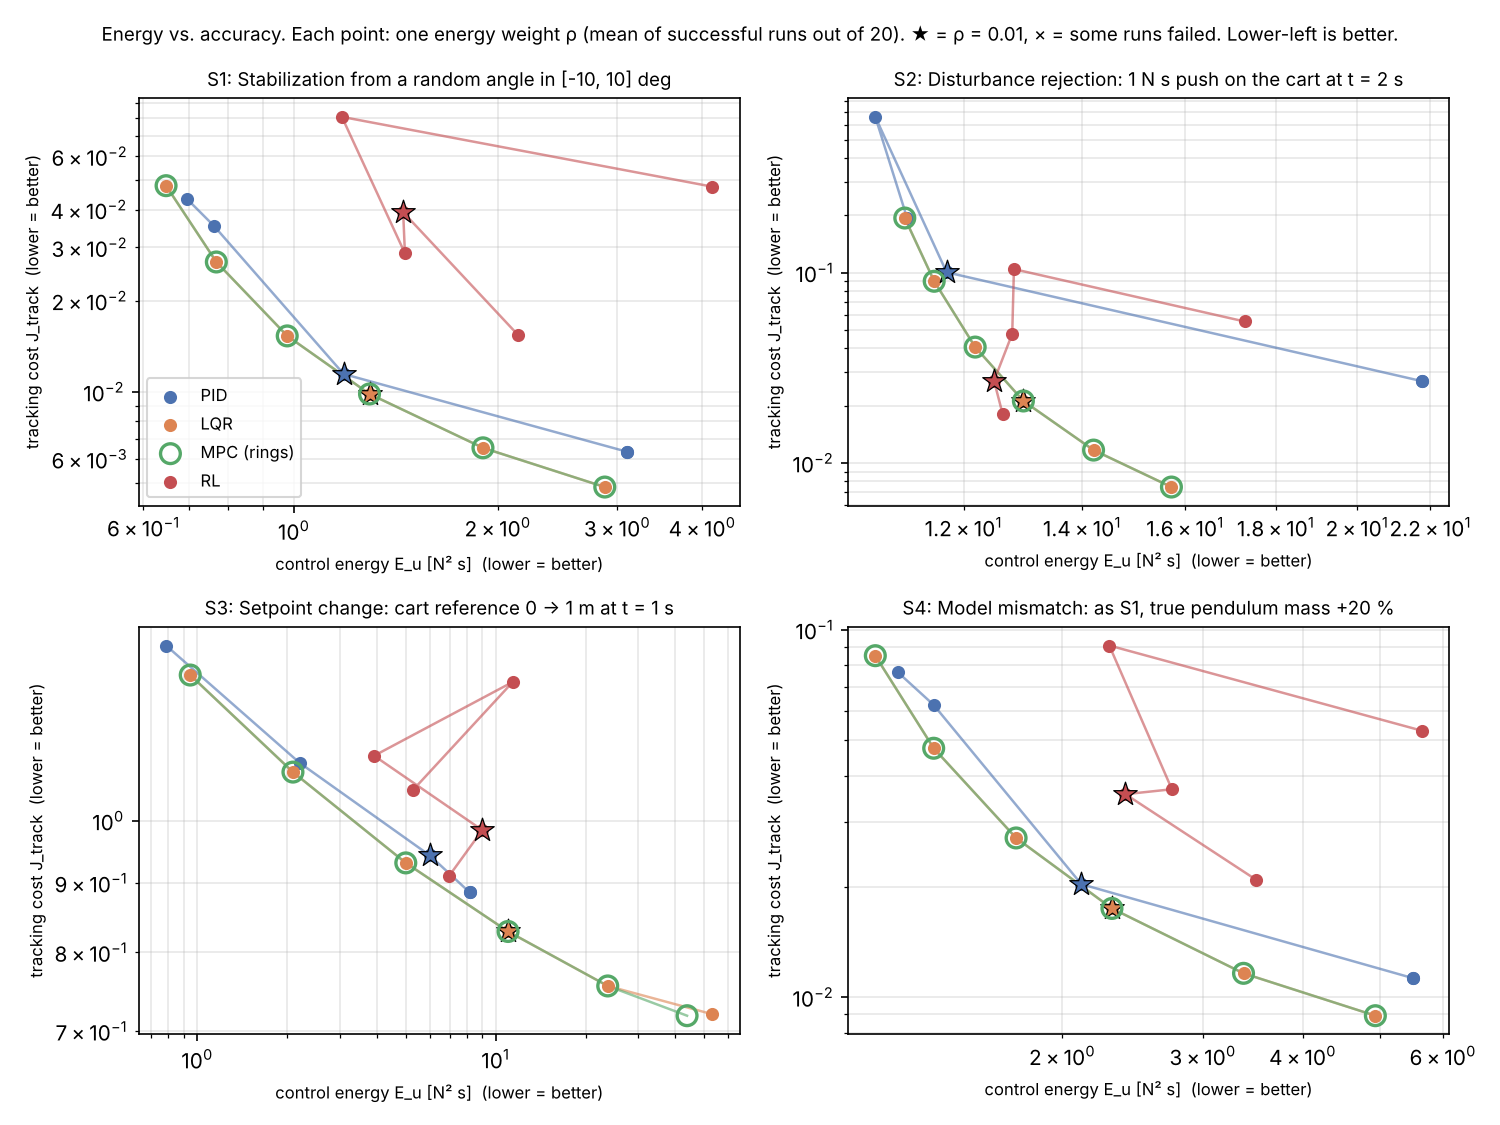
\includegraphics[width=0.86\textwidth]{eval/pareto.png}
\caption{Energy--accuracy Pareto fronts. Each point is one energy weight
$\rho$ (mean of 20 runs); stars mark $\rho=0.01$. MPC (rings) coincides
with LQR. Lower-left is better.}
\label{fig:pareto}
\end{figure*}

\section{Controllers}
All controllers share the interface $u=\mathrm{controller}(s,t)$ and are
tuned for the same continuous cost
\begin{equation}
J = \underbrace{\int_0^T (x-x_\mathrm{ref})^2+\theta^2\,dt}_{J_\mathrm{track}}
\;+\;\rho\underbrace{\int_0^T u^2\,dt}_{E_u},\label{eq:cost}
\end{equation}
for $\rho\in\{0.001,0.003,0.01,0.03,0.1,0.3\}$; $\rho=0.01$ is the main
setting.

\textbf{PID (cascaded).} An outer PD loop turns the cart error into a lean
command, $\theta_\mathrm{ref}=-(k_x e_x+k_v\dot x)$, clipped to $\pm10^\circ$
(to move right, the pendulum must first lean right). An inner PID on
$e=\theta-\theta_\mathrm{ref}$ gives $u=k_pe+I+k_d\dot\theta$ with
back-calculation anti-windup ($\dot I = k_ie + (u_\mathrm{sat}-u)/T_t$,
$T_t=0.1$\,s). After a manual start ($k_p=30$, $k_d=4$, $k_x=0.1$, $k_v=0.2$:
oscillatory, $E_u=106$\,N$^2$s on the tuning set) the gains were chosen by an
800-point grid search on 10 tuning initial conditions. For $\rho=0.01$ the
grid search selects $k_p=50$, $k_d=11$, $k_x=0.18$, $k_v=0.15$, $k_i=0$.
With full state measurement, this cascade is a static state feedback
$u = k_p\theta + k_d\dot\theta + k_pk_x e_x + k_pk_v\dot x$, and the selected
gains are close to the LQR gains below. The integral term never improved the
cost (no constant disturbance acts on this frictionless system).

\textbf{LQR.} Discrete LQR on $(A_d,B_d)$ with $Q_d=Q\Delta t$,
$Q=\mathrm{diag}(1,0,1,0)$, $R_d=\rho\Delta t$, the discrete equivalent of
\eqref{eq:cost}. For $\rho=0.01$:
$K=[-8.70,\,-8.20,\,-48.72,\,-10.60]$, $u=-K(s-s_\mathrm{ref})$.

\textbf{MPC.} Linear MPC with horizon $N$ on the same model and cost, the
Riccati matrix $P$ of the LQR as terminal weight, $|u_k|\le10$\,N and a soft
track constraint $|x_k|\le 2.35$\,m (5\,cm margin; slack penalized
quadratically and linearly so the QP is always feasible). States are
eliminated, leaving a dense QP with $N+1$ variables, solved by qpOASES through
CasADi with warm starts. The energy term $\rho\,u^2$ is explicit in the cost.
Only the current reference is used (no preview of future setpoints).

\textbf{RL (SAC).} A custom Gymnasium environment wraps our simulator;
observation $[x-x_\mathrm{ref},\dot x,\theta,\dot\theta]$, action
$a\in[-1,1]$, $u=10a$. Reward (v2):
$r=\max\!\bigl(0,\,1-\beta\,[(x-x_\mathrm{ref})^2+\theta^2+\rho u^2]\bigr)$ with
$\beta=5$, and $-100$ when the pendulum exceeds $30^\circ$ or the cart leaves
the track, so the energy penalty uses the same $\rho$ as the other methods.
Training randomizes the initial state ($|x_0-x_\mathrm{ref}|\le1$\,m,
$|\theta_0|\le12^\circ$, velocities $\le0.5$) and, in half of the episodes,
applies a random 0.5--1.2\,N\,s push. SAC (Stable-Baselines3, $2\times128$
MLP, $\gamma=0.995$, 150k steps, fixed seeds) was trained for
$\rho\in\{0.001,0.01,0.03,0.1,0.3\}$, plus two extra seeds at $\rho=0.01$.
For each run, the best of the 50k, 100k and 150k-step checkpoints on the
tuning set is used.

\section{Experimental Setup}
Four scenarios of 10\,s each, 20 random initial conditions per scenario,
drawn from a seed never used for tuning or training:
\textbf{S1} start at $\theta_0\sim\mathcal U(-10^\circ,10^\circ)$, cart at
rest; \textbf{S2} near-upright start ($|\theta_0|\le2^\circ$) and a 1\,N\,s
push (20\,N for 50\,ms) on the cart at $t=2$\,s; \textbf{S3} cart reference
steps from 0 to 1\,m at $t=1$\,s; \textbf{S4} as S1 but the true pendulum
mass is 20\,\% higher than every controller assumes. A run fails if
$|\theta|>30^\circ$ or $|x|>2.4$\,m. Metrics: $E_u=\int u^2dt$,
$E_\mathrm{mech}=\int|u\dot x|dt$, $J_\mathrm{track}$, angle settling time
$t_s$ (into $\pm1^\circ$, measured from the push/step in S2/S3), maximum
angle, cart overshoot (S3), success rate and controller computation time per
step (Python, one CPU core). Means and standard deviations are over
successful runs. Energy differences are tested against LQR with a paired
Wilcoxon signed-rank test on the same initial conditions.

\begin{table*}[t]
\centering\small
\caption{Main results at $\rho=0.01$: mean\,$\pm$\,std over 20 initial
conditions per scenario (all runs successful). $t_s$: settling time of the
angle into $\pm1^\circ$; $t_c$: controller computation time per step.
Cart overshoot in S3: \overshoottext.}
\label{tab:main}
\resizebox{\textwidth}{!}{\begin{tabular}{llrrrrrrr}
\toprule
Sc. & Ctrl. & $E_u$ [N$^2$s] & $E_\mathrm{mech}$ [J] & $J_\mathrm{track}$ & $t_s$ [s] & $\theta_\mathrm{max}$ [$^\circ$] & Succ. [\%] & $t_c$ [ms] \\
\midrule
S1 & PID & 1.18\,$\pm$\,1.16 & 0.115\,$\pm$\,0.113 & 0.011\,$\pm$\,0.011 & 0.85\,$\pm$\,0.72 & 4.0\,$\pm$\,2.8 & 100 & 0.010 \\
 & LQR & 1.29\,$\pm$\,1.27 & 0.123\,$\pm$\,0.121 & 0.010\,$\pm$\,0.010 & 0.66\,$\pm$\,0.51 & 4.0\,$\pm$\,2.8 & 100 & 0.004 \\
 & MPC & 1.29\,$\pm$\,1.27 & 0.123\,$\pm$\,0.121 & 0.010\,$\pm$\,0.010 & 0.66\,$\pm$\,0.51 & 4.0\,$\pm$\,2.8 & 100 & 0.295 \\
 & RL & 1.45\,$\pm$\,1.45 & 0.108\,$\pm$\,0.109 & 0.039\,$\pm$\,0.040 & 1.84\,$\pm$\,1.74 & 4.0\,$\pm$\,2.8 & 100 & 0.137 \\
\midrule
S2 & PID & 11.74\,$\pm$\,0.11 & 0.718\,$\pm$\,0.012 & 0.101\,$\pm$\,0.003 & 1.38\,$\pm$\,0.01 & 6.6\,$\pm$\,0.1 & 100 & 0.012 \\
 & LQR & 12.97\,$\pm$\,0.09 & 0.802\,$\pm$\,0.009 & 0.021\,$\pm$\,0.001 & 1.14\,$\pm$\,0.01 & 6.7\,$\pm$\,0.1 & 100 & 0.002 \\
 & MPC & 12.97\,$\pm$\,0.09 & 0.802\,$\pm$\,0.009 & 0.021\,$\pm$\,0.001 & 1.14\,$\pm$\,0.01 & 6.7\,$\pm$\,0.1 & 100 & 0.303 \\
 & RL & 12.48\,$\pm$\,0.16 & 0.678\,$\pm$\,0.014 & 0.027\,$\pm$\,0.002 & 2.22\,$\pm$\,0.02 & 6.3\,$\pm$\,0.2 & 100 & 0.171 \\
\midrule
S3 & PID & 6.01\,$\pm$\,0.06 & 1.531\,$\pm$\,0.018 & 0.943\,$\pm$\,0.012 & 2.53\,$\pm$\,0.01 & 8.9\,$\pm$\,0.0 & 100 & 0.009 \\
 & LQR & 11.00\,$\pm$\,0.11 & 1.847\,$\pm$\,0.006 & 0.829\,$\pm$\,0.013 & 2.24\,$\pm$\,0.00 & 12.0\,$\pm$\,0.1 & 100 & 0.002 \\
 & MPC & 11.00\,$\pm$\,0.11 & 1.847\,$\pm$\,0.006 & 0.829\,$\pm$\,0.013 & 2.24\,$\pm$\,0.00 & 12.0\,$\pm$\,0.1 & 100 & 0.291 \\
 & RL & 9.01\,$\pm$\,0.79 & 1.513\,$\pm$\,0.041 & 0.984\,$\pm$\,0.030 & 3.21\,$\pm$\,0.02 & 7.5\,$\pm$\,0.1 & 100 & 0.119 \\
\midrule
S4 & PID & 2.11\,$\pm$\,1.71 & 0.206\,$\pm$\,0.167 & 0.020\,$\pm$\,0.016 & 1.29\,$\pm$\,0.89 & 5.5\,$\pm$\,3.4 & 100 & 0.010 \\
 & LQR & 2.31\,$\pm$\,1.87 & 0.220\,$\pm$\,0.179 & 0.017\,$\pm$\,0.014 & 1.02\,$\pm$\,0.70 & 5.5\,$\pm$\,3.4 & 100 & 0.002 \\
 & MPC & 2.31\,$\pm$\,1.87 & 0.220\,$\pm$\,0.179 & 0.017\,$\pm$\,0.014 & 1.02\,$\pm$\,0.70 & 5.5\,$\pm$\,3.4 & 100 & 0.307 \\
 & RL & 2.40\,$\pm$\,1.98 & 0.192\,$\pm$\,0.156 & 0.036\,$\pm$\,0.032 & 1.69\,$\pm$\,1.19 & 5.5\,$\pm$\,3.4 & 100 & 0.108 \\
\bottomrule
\end{tabular}
}
\end{table*}

\section{Results}
\begin{figure}[t]
\centering
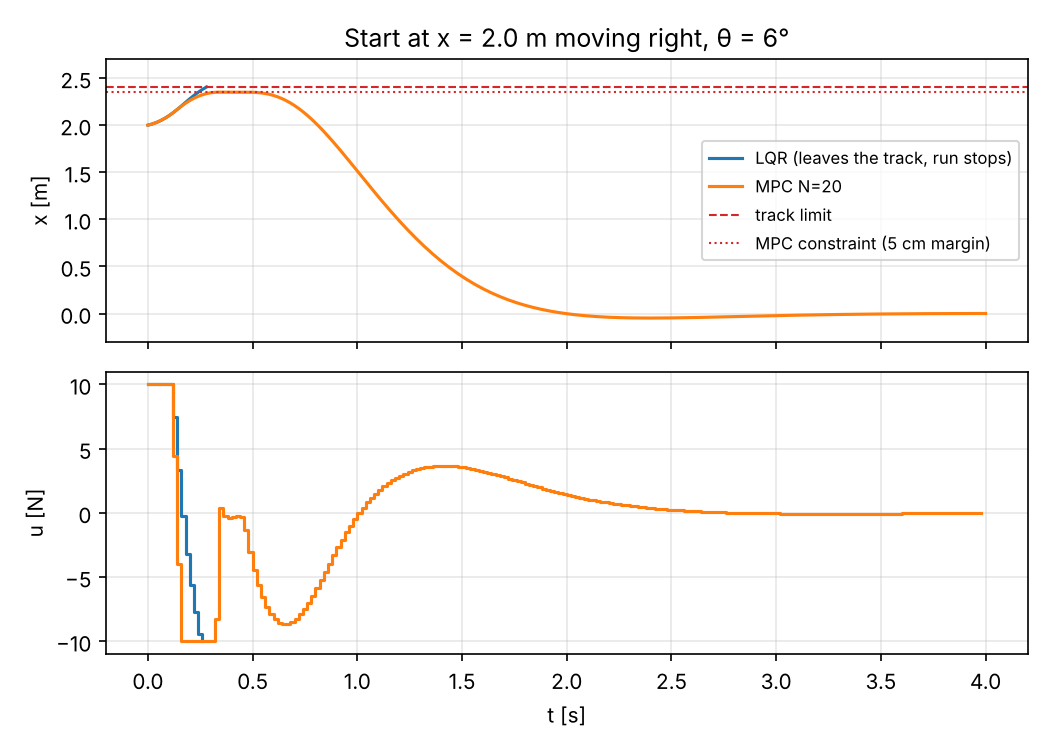
\includegraphics[width=\columnwidth]{mpc/track_constraint.png}
\caption{Start at $x=2.0$\,m moving right: LQR leaves the track, MPC brakes
at its 2.35\,m constraint and returns.}
\label{fig:track}
\end{figure}

\begin{figure}[t]
\centering
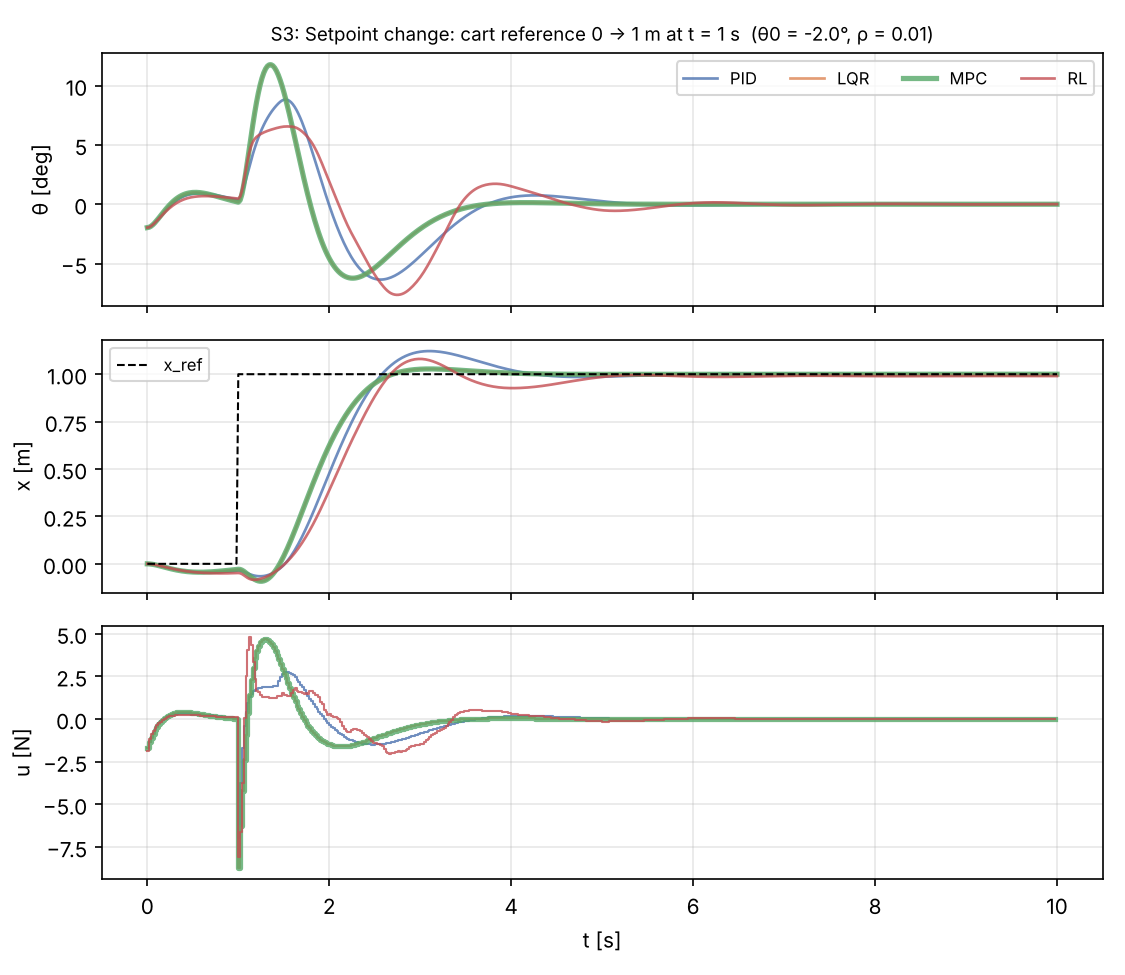
\includegraphics[width=\columnwidth]{eval/traj_S3.png}
\caption{S3 (reference step at $t=1$\,s), $\rho=0.01$. LQR lies under the
MPC curve. PID and RL use less force but overshoot more.}
\label{fig:traj}
\end{figure}


\textbf{Overall.} All four controllers balanced the pendulum in all
$4\times20$ evaluation runs at every energy weight (Table~\ref{tab:main}).
Fig.~\ref{fig:pareto} shows the energy--accuracy fronts; Table~\ref{tab:paired}
compares each controller with LQR on the same initial conditions.

\textbf{LQR and MPC define the front.} In every scenario the LQR points form
the lower-left boundary. MPC produces exactly the same trajectories as LQR.
This is not a bug but a property of the design: with the Riccati matrix as
terminal weight, an unconstrained linear MPC \emph{is} the LQR. In the four
scenarios the track is never approached ($|x|\le1.03$\,m) and the force limit
is active only for a few samples during the push (LQR requests up to
11.9\,N); there, the optimal constrained input equals the clipped LQR input.
MPC costs about 0.3\,ms per step against 0.003\,ms for LQR, both far below
the 20\,ms period.

\textbf{PID.} At $\rho=0.01$ the tuned PID uses 8--46\,\% less energy than
LQR (Table~\ref{tab:paired}) but is less accurate in every scenario (tracking
cost $\times1.14$ to $\times4.8$, overshoot 12\,\% vs.\ 2.7\,\% in S3,
Fig.~\ref{fig:traj}). At
equal energy, its tracking cost is 1.01--1.42$\times$ that of the LQR front for
$\rho=0.01$, and up to 3.6$\times$ for extreme weights, where the coarse grid
limits it. The saving is therefore bought with accuracy, not obtained for
free.

\textbf{RL.} At $\rho=0.01$ the SAC policy used 10\,\% \emph{more} energy
than LQR in S1 with a $3.9\times$ higher tracking cost, and in S4 12\,\% more
energy (not significant, $p=0.37$) with $1.6\times$ the tracking cost. At
equal energy it needs 2.6--9.8$\times$ (S1) and 1.8--6.0$\times$ (S4) the
tracking cost of the LQR front. S2 is the exception: here RL lies \emph{beyond}
the LQR front. The agent trained with $\rho=0.001$ used 3\,\% less energy
than LQR ($\rho=0.01$) with 17\,\% lower tracking cost (paired Wilcoxon,
$p<0.001$). S2 is the one scenario whose disturbance type (a short push) was
part of RL training, while LQR is optimal only for the undisturbed linear
model. RL also delivered the least \emph{mechanical} energy in all four
scenarios (e.g.\ S2: 0.68\,J vs.\ 0.80\,J for LQR). The energy weight does
not map monotonically to RL behavior: the $\rho=0.3$ agent used more energy
than the $\rho=0.1$ agent, and its learning curve had not converged after
150k steps.

\begin{table}[t]
\centering\small
\caption{Paired comparison with LQR at $\rho=0.01$: median ratio over the 20
initial conditions and Wilcoxon $p$-value for the energy difference.}
\label{tab:paired}
\begin{tabular}{llrrr}
\toprule
Sc. & Ctrl. & $E_u$ ratio & $J_\mathrm{track}$ ratio & $p$ (Wilcoxon) \\
\midrule
S1 & PID & 0.92 & 1.16 & $<$0.001 \\
S1 & MPC & 1.00 & 1.00 & -- \\
S1 & RL & 1.10 & 3.88 & 0.033 \\
S2 & PID & 0.90 & 4.81 & $<$0.001 \\
S2 & MPC & 1.00 & 1.00 & -- \\
S2 & RL & 0.96 & 1.28 & $<$0.001 \\
S3 & PID & 0.54 & 1.14 & $<$0.001 \\
S3 & MPC & 1.00 & 1.00 & -- \\
S3 & RL & 0.84 & 1.18 & $<$0.001 \\
S4 & PID & 0.92 & 1.16 & $<$0.001 \\
S4 & MPC & 1.00 & 1.00 & -- \\
S4 & RL & 1.12 & 1.64 & 0.368 \\
\bottomrule
\end{tabular}

\end{table}

\textbf{Robustness (S4).} With a 20\,\% heavier pendulum, all controllers
still succeeded in every run; the LQR tracking cost rose from 0.010 (S1) to
0.017 and energy from 1.29 to 2.31\,N$^2$s, with the same ranking as in S1.

\textbf{MPC horizon.} Table~\ref{tab:horizon} uses the tuning set. With the
Riccati terminal weight, $N=10$, 20 and 40 give identical closed loops; the
solve time grows from 0.24 to 0.58\,ms. Without a terminal weight, $N=10$
(0.2\,s) and $N=20$ (0.4\,s) are shorter than the dynamics need and fail in
every run; $N=40$ stabilizes but is 50\,\% less accurate.

\begin{table}[t]
\centering\small
\caption{MPC horizon study ($\rho=0.01$, 10 tuning initial conditions).}
\label{tab:horizon}
\begin{tabular}{lrrrrr}
\toprule
Terminal cost & $N$ & $J_\mathrm{track}$ & $E_u$ & Fails & $t_c$ [ms] \\
\midrule
Riccati $P$ & 10 & 0.0827 & 2.74 & 0/10 & 0.244 \\
Riccati $P$ & 20 & 0.0827 & 2.74 & 0/10 & 0.341 \\
Riccati $P$ & 40 & 0.0827 & 2.74 & 0/10 & 0.581 \\
none & 10 & -- & -- & 10/10 & 0.284 \\
none & 20 & -- & -- & 10/10 & 0.384 \\
none & 40 & 0.1238 & 1.61 & 0/10 & 0.610 \\
LQR (no MPC) & -- & 0.0827 & 2.74 & 0/10 & 0.002 \\
\bottomrule
\end{tabular}

\end{table}

\textbf{When constraints matter.} A supplementary test starts the cart at
$x_0\in\{1.4,\dots,2.0\}$\,m moving towards the track end (36 starts,
$|\theta_0|\le10^\circ$). Success: LQR 14/36, MPC 19/36 (same for $N=40$),
PID 24/36, RL 30/36. MPC keeps the cart on the track where LQR leaves it
(Fig.~\ref{fig:track}), but the linear prediction model limits how much it can
gain. PID benefits from its $10^\circ$ lean limit, and RL from having learned
the track ends from the episode terminations.

\begin{figure}[t]
\centering
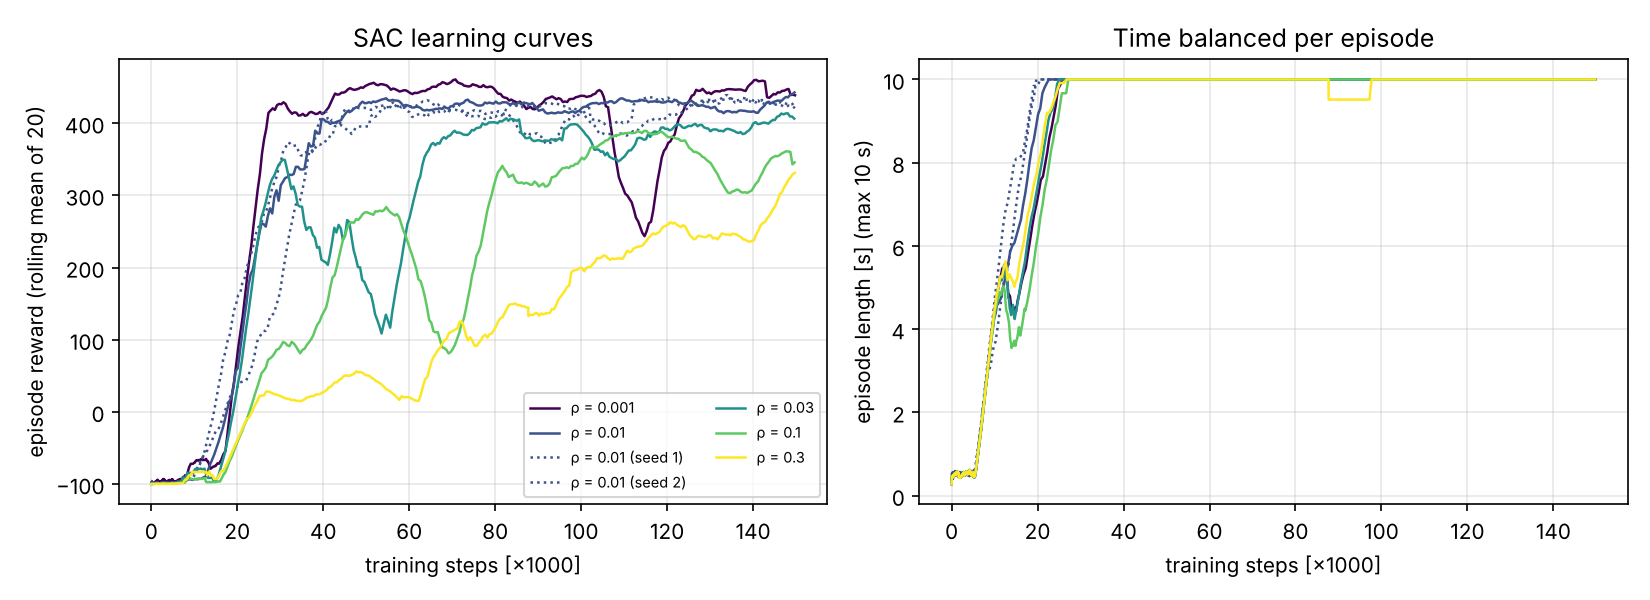
\includegraphics[width=\columnwidth]{rl/learning_curves.png}
\caption{SAC learning curves (reward v2). All agents balance for the full
10\,s after about 25k steps; larger energy weights learn more slowly.}
\label{fig:lc}
\end{figure}

\textbf{RL reward design and variability.} The first reward
($\beta=1$, no clipping, $\gamma=0.99$) produced a policy that balanced
perfectly but stopped with the cart 19\,cm from the reference: near the
reference, the quadratic position penalty was too small to justify leaning
the wrong way first, and a 2\,s horizon was too short to see the benefit
(S1 tracking cost 0.317). Scaling the cost ($\beta=5$), clipping the reward at
zero and $\gamma=0.995$ reduced the offset to 1--3\,cm. Checkpoints at 50k,
100k and 150k steps were compared on the tuning set; the final model was
selected in 5 of 7 runs. Across three seeds at $\rho=0.01$, the S1 tracking
cost ranged from 0.019 to 0.039 and the S3 energy from 8.8 to
10.4\,N$^2$s, a spread far larger than for the deterministic designs.
Each agent took about 17\,min of training on one CPU core.

\section{Discussion}
\textbf{Which controller wins?} For the question we posed, the most
energy-efficient control at comparable accuracy, \emph{LQR} wins: it sits on
the Pareto front in every scenario, is the simplest to design and the
cheapest to run. This is expected, since our shared cost is quadratic and the
pendulum stays in a nearly linear range ($|\theta|\le12^\circ$), so LQR is the
optimal solution of exactly this problem for the undisturbed model. MPC
matches LQR and adds value only where constraints bind, as near the track
end. The tuned PID is a good baseline whose structure is equivalent to state
feedback, but its energy savings come with lower accuracy. RL needs no model
at run time and handled pushes and track ends best, but needed a reward
redesign (Fig.~\ref{fig:lc}), shows large seed-to-seed variation and does not reach the front in
nominal regulation.

\textbf{Limitations.} Point-mass pendulum, no friction, no sensor noise or
delay, full state measurement; MPC is linear (nonlinear MPC was not
implemented); RL used a single training budget of 150k steps and was the only
method trained with pushes, which favors it in S2; computation times are
Python wall times on one core; the fall threshold of $30^\circ$ is our
choice.

\section{Conclusion}
On a validated nonlinear cart-pole simulator with a common cost and identical
test conditions, LQR provides the best energy--accuracy trade-off;
linear MPC with an LQR terminal weight reproduces it and is only worth its
100$\times$ higher computation when constraints are active; a grid-searched
PID comes close; and SAC is competitive under disturbances it was trained on
but otherwise needs 2--10$\times$ the tracking error for the same energy.
Natural next steps are nonlinear MPC, sensor noise and delay, and deployment
on embedded hardware.

\textbf{Reproducibility.} All results follow from the repository with fixed
seeds (evaluation seed 2026, tuning seed 7, RL seeds 0--2); see
\texttt{README.md} for the commands. AI coding tools were used for help with parts
of the code.

\small
\begin{thebibliography}{9}\setlength{\itemsep}{0pt}
\bibitem{barto83} A.~G. Barto, R.~S. Sutton, C.~W. Anderson, ``Neuronlike adaptive elements that can solve difficult learning control problems,'' \emph{IEEE Trans.\ SMC}, 1983.
\bibitem{astrom} K.~J. \AA str\"om, R.~M. Murray, \emph{Feedback Systems}, 2nd ed., Princeton Univ.\ Press, 2021.
\bibitem{rawlings} J.~B. Rawlings, D.~Q. Mayne, M.~Diehl, \emph{Model Predictive Control: Theory, Computation, and Design}, 2nd ed., Nob Hill, 2017.
\bibitem{casadi} J.~A.~E. Andersson et al., ``CasADi: a software framework for nonlinear optimization and optimal control,'' \emph{Math.\ Prog.\ Comp.}, 2019.
\bibitem{qpoases} H.~J. Ferreau et al., ``qpOASES: a parametric active-set algorithm for quadratic programming,'' \emph{Math.\ Prog.\ Comp.}, 2014.
\bibitem{sutton} R.~S. Sutton, A.~G. Barto, \emph{Reinforcement Learning: An Introduction}, 2nd ed., MIT Press, 2018.
\bibitem{sac} T.~Haarnoja et al., ``Soft actor-critic: off-policy maximum entropy deep RL with a stochastic actor,'' ICML, 2018.
\bibitem{sb3} A.~Raffin et al., ``Stable-Baselines3: reliable reinforcement learning implementations,'' \emph{JMLR}, 2021.
\end{thebibliography}

\end{document}
